\chapter{Compiler and Code Optimization}
\label{ch:compiler-optimization}

\section{Introduction}

A compiler is a program that translates source code written in a high-level programming language into machine code executable by a processor. This translation is not a straightforward one-to-one mapping: modern compilers perform extensive analysis and transformation of the program to produce code that executes faster, consumes less energy, or occupies less memory. These transformations are collectively referred to as \textit{code optimizations}.

The importance of compiler optimization has grown alongside the complexity of both hardware and software. Modern processors feature deep cache hierarchies, wide \gls{simd} units, and multiple cores, each introducing new opportunities and constraints for program optimization. Simultaneously, software workloads, particularly in machine learning, have grown in scale and computational intensity, making the quality of compiled code a critical factor in overall system performance.

\section{Phases of a Compiler: From Source Code to Executable}

A compiler typically operates in three major phases: the \textit{front-end}, the \textit{middle-end}, and the \textit{back-end}~\cite{aho2006compilers}. Each phase transforms the program into a progressively lower-level representation, as illustrated in the standard compilation pipeline shown in Figure~\ref{fig:compiler-pipeline}.

\begin{figure}[H]
    \centering
    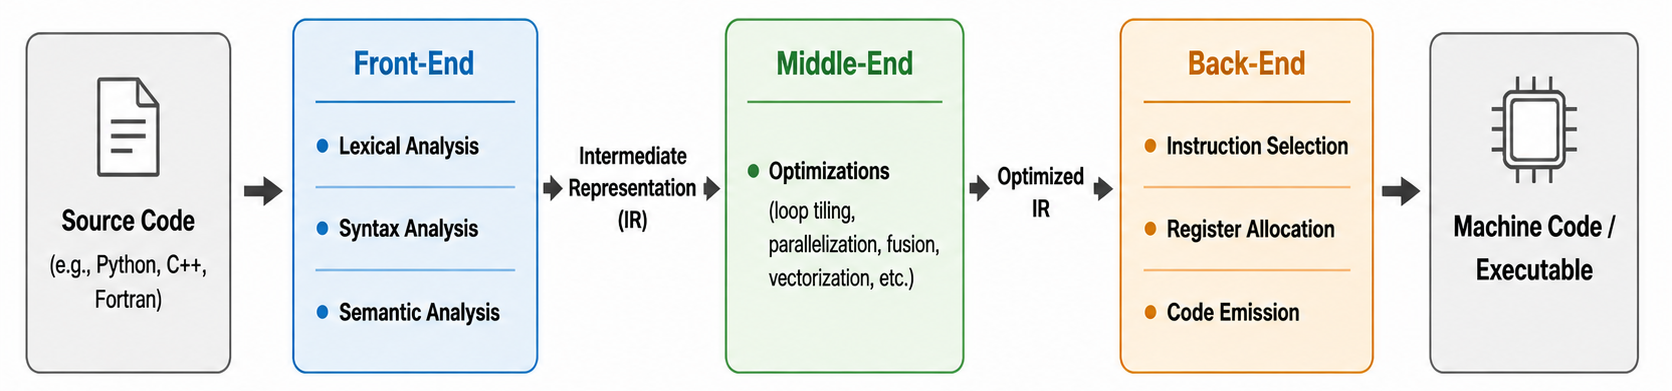
\includegraphics[width=1.0\textwidth]{ressources/chapter1/compiler_phases.png}
    \caption{The three phases of a compiler.}
    \label{fig:compiler-pipeline}
\end{figure}

\subsection{Front-End}

The front-end is responsible for reading the source code and converting it into an \gls{ir}. This process involves three sub-steps:

\begin{itemize}
    \item \textbf{Lexical analysis} (scanning): The source text is broken into tokens, keywords, identifiers, literals, and operators. For instance, the expression \texttt{x = a + 2} is tokenized into \texttt{IDENT(x)}, \texttt{ASSIGN}, \texttt{IDENT(a)}, \texttt{PLUS}, \texttt{INT(2)}.
    \item \textbf{Syntax analysis} (parsing): The sequence of tokens is organized into a parse tree or \gls{ast} according to the grammar of the source language. This step verifies that the program is syntactically well-formed.
    \item \textbf{Semantic analysis}: The compiler checks for semantic correctness, type compatibility, variable declarations before use, scope rules, and annotates the \gls{ast} with type information and symbol table entries.
\end{itemize}

The output of the front-end is an \gls{ir}, typically in a form such as three-address code or \gls{ssa} form. \gls{ssa} is a representation where each variable is assigned exactly once, which simplifies many subsequent analyses and transformations.

\subsection{Middle-End}

The middle-end operates on the \gls{ir} and is where the majority of optimizations take place. Because the \gls{ir} is independent of both the source language and the target machine, optimizations at this level are portable and can be shared across different language front-ends and hardware back-ends. Middle-end optimizations include:

\begin{itemize}
    \item \textbf{Control-flow optimizations}: constant propagation, dead code elimination, loop-invariant code motion.
    \item \textbf{Data-flow optimizations}: common subexpression elimination, copy propagation, strength reduction.
    \item \textbf{Loop optimizations}: tiling, fusion, interchange, unrolling, vectorization.
    \item \textbf{Inter-procedural optimizations}: function inlining, inter-procedural constant propagation.
\end{itemize}

Automated optimization research and modern machine learning compilation frameworks predominantly focus on this middle-end level, leveraging structured abstractions like the \gls{mlir} Linalg dialect to apply structural optimizations to tensor and algebra pipelines before downstream code generation.

\newpage
\subsection{Back-End}

The back-end translates the optimized \gls{ir} into machine code for a specific target architecture. This phase includes:

\begin{itemize}
    \item \textbf{Instruction selection}: mapping \gls{ir} operations to target machine instructions, often using pattern-matching techniques on a tree representation of the \gls{ir}.
    \item \textbf{Instruction scheduling}: reordering instructions to exploit instruction-level parallelism and avoid pipeline stalls.
    \item \textbf{Register allocation}: assigning program variables to the limited set of physical registers, spilling to memory when necessary.
    \item \textbf{Code emission}: generating the final assembly or object code.
\end{itemize}

While the back-end performs critical target-dependent transformations, high-level loop optimization strategies typically focus on the middle-end, where structural changes yield the largest impact on memory access patterns and hardware parallelism.

\section{Optimization Paradigms and Techniques}
\label{sec:opt-paradigms}

Compiler optimizations can be categorized along several axes, and they are supported by fundamental program analysis techniques.

\subsection{Machine-Dependent vs. Machine-Independent Optimization}

Optimizations are classified as \textit{machine-independent} when they improve the program without knowledge of the target hardware, and \textit{machine-dependent} when they exploit specific hardware features.

Machine-independent optimizations include constant folding (evaluating constant expressions at compile time), dead code elimination (removing computations whose results are never used), and common subexpression elimination (reusing previously computed values). These transformations are universally beneficial and apply regardless of the target architecture.

Machine-dependent optimizations, by contrast, require knowledge of the target processor. Examples include selecting vector instructions matching the \gls{simd} width of the \gls{cpu}, choosing tile sizes that fit within a specific cache level, and scheduling instructions to match the pipeline depth of a particular micro-architecture.

\newpage
\subsection{Static vs.\ Dynamic Optimization}

Optimizations can also be classified by when they are applied. \textit{Static optimization} occurs at compile time, before the program executes. The compiler analyzes the source code or \gls{ir} and applies transformations based on information available statically. Most traditional compiler optimizations fall into this category.

\textit{Dynamic optimization} occurs at runtime, during program execution. \gls{jit} compilers monitor program behavior and apply optimizations based on observed execution patterns. Dynamic optimization can exploit runtime information, such as branch frequencies, hot paths, and actual data values, that is unavailable at compile time. The trade-off is that the optimization itself consumes runtime resources.

\subsection{Control-Flow and Data-Flow Analysis}

Before applying any transformation, the compiler must analyze the program to determine whether the transformation is legal and to estimate whether it will be beneficial. Two families of analysis form the foundation of most compiler optimizations.

\textbf{Control-flow analysis} constructs a representation of the possible execution paths through the program. The most common representation is the \gls{cfg}, where nodes represent \textit{basic blocks}, maximal sequences of instructions with a single entry and a single exit, and edges represent possible transfers of control (branches, jumps, fall-through). As demonstrated by the structural example in Figure~\ref{fig:cfg-example}, the \gls{cfg} enables the compiler to reason about dominance (which blocks must execute before others), loops and reachability.

\begin{figure}[H]
    \centering
    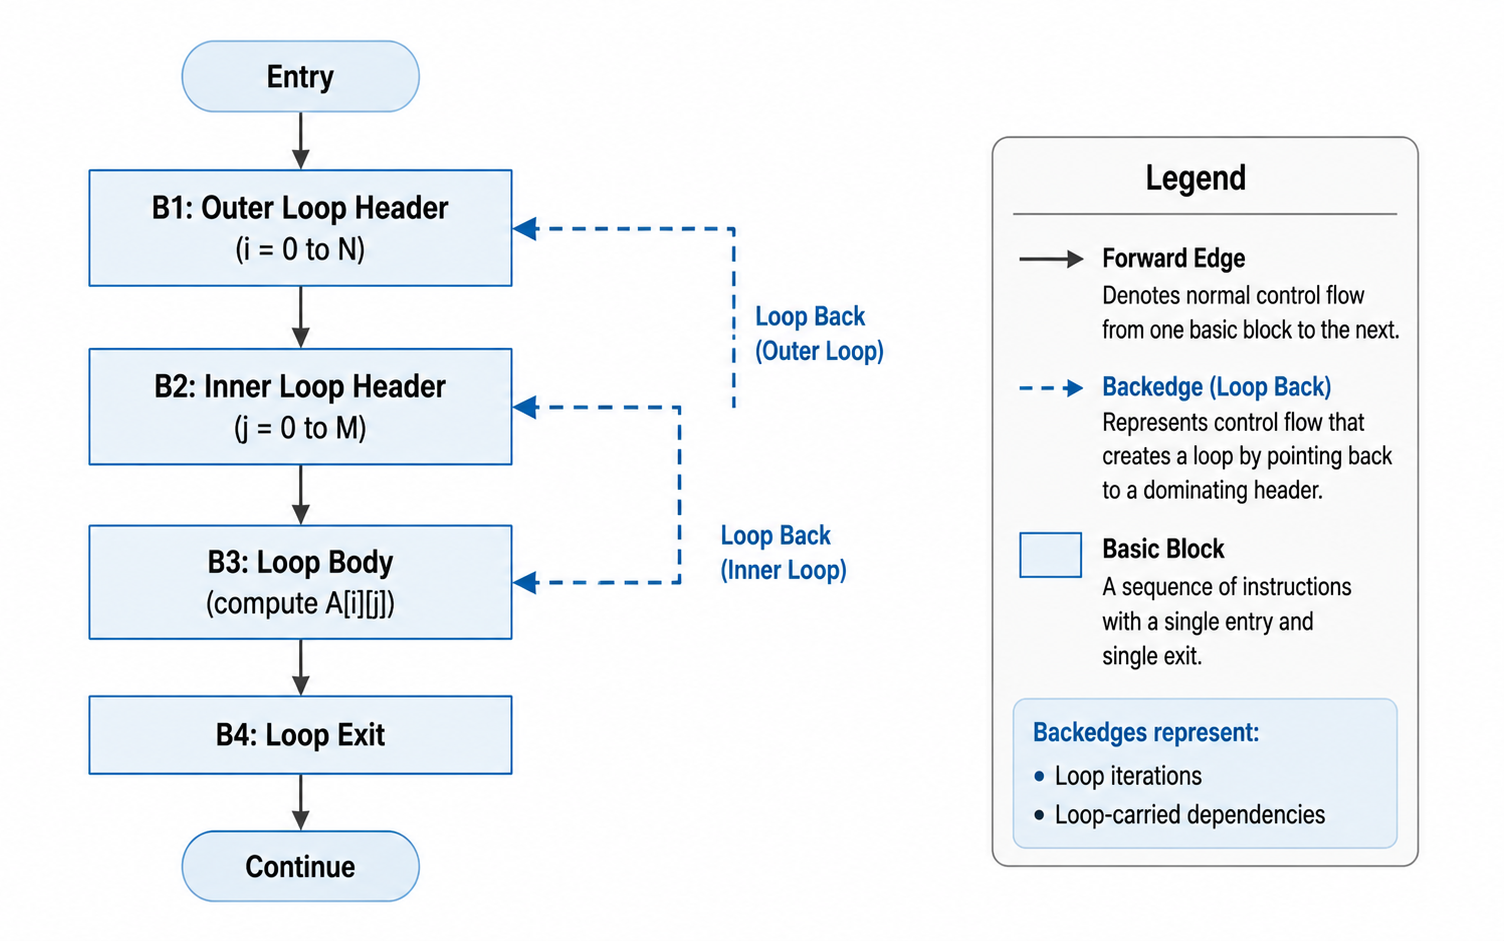
\includegraphics[width=0.8\textwidth]{ressources/chapter1/control_flow_graph.png}
    \caption{Example of a control-flow graph for a nested loop structure}
    \label{fig:cfg-example}
\end{figure}

\textbf{Data-flow analysis} determines how values are defined, used, and propagated through the program. Key data-flow problems include:

\begin{itemize}
    \item \textbf{Reaching definitions}: For each program point, which assignments to a variable may have reached that point without being overwritten? This analysis supports constant propagation and common subexpression elimination.
    \item \textbf{Live variable analysis}: For each program point, which variables hold values that may be read before being overwritten? This analysis supports register allocation and dead code elimination.
    \item \textbf{Available expressions}: Which expressions have already been computed and not invalidated? This supports global common subexpression elimination.
\end{itemize}

These analyses are typically formulated as iterative fixed-point computations over a lattice of data-flow facts. In modern multi-level intermediate representations, dependency analyses for loop transformations are frequently augmented by specialized multi-dimensional infrastructure or polyhedral representation abstractions.

\section{Loop Nest Optimization}

Loops account for the vast majority of execution time in compute-intensive programs, particularly in scientific computing and machine learning workloads. A \textit{loop nest} is a set of loops where one loop is contained within the body of another. For example, matrix multiplication involves three nested loops iterating over rows, columns, and the inner product dimension. Optimizing loop nests is therefore one of the most impactful activities an optimizing compiler can perform.

This section describes the primary loop nest transformations used in modern optimizing compilers. For each transformation, we outline its definition and execution mechanics, its equivalent representation within the \gls{mlir}-\gls{rl} optimization framework, and its foundational microarchitectural performance benefits.

\subsection{Parallelization}

Parallelization distributes the iterations of a loop across multiple processing units, such as \gls{cpu} cores or hardware threads, so that they execute concurrently rather than sequentially. This is achieved by verifying that iterations are completely independent, meaning no iteration reads from or writes to a memory location that is modified by a separate, concurrent iteration. 

In the \gls{mlir}-\gls{rl} framework established in prior work~\cite{bendib2024reinforcement}, this optimization is represented by the \gls{tp} action or the composite \gls{tf} action.

\begin{itemize}
    \item \textbf{Accelerated Wall-Clock Time:} Exploits multi-core processing architectures to scale execution throughput linearly with available hardware threads.
    \item \textbf{Optimized Resource Utilization:} Minimizes execution hotspots by balancing computational workloads evenly across independent processing elements.
\end{itemize}

\subsection{Interchange (Permutation)}

Loop interchange swaps the structural nesting order of loops, modifying which iterator sits outermost and which operates innermost. This transformation is applied by rearranging the loop control indices, provided that the data dependence vectors of the original loop nest remain lexicographically positive under the new iteration order.

In \gls{mlir}-\gls{rl} of prior works, this transformation corresponds to the \gls{i} action, which evaluates and selects an optimal loop order from the $D!$ possible permutations of a depth-$D$ nest. The operational impact of this stride re-alignment on underlying memory access layouts is illustrated in Figure~\ref{fig:loop-interchange}.

\begin{itemize}
    \item \textbf{Maximized Spatial Locality:} Aligns the fastest-moving inner loop iterator with the contiguous memory layout (e.g., row-major order) of target arrays.
    \item \textbf{Reduced Pipeline Stalls:} Enhances the efficacy of hardware prefetchers, dramatically lowering data-cache miss rates.
\end{itemize}

\begin{figure}[H]
    \centering
    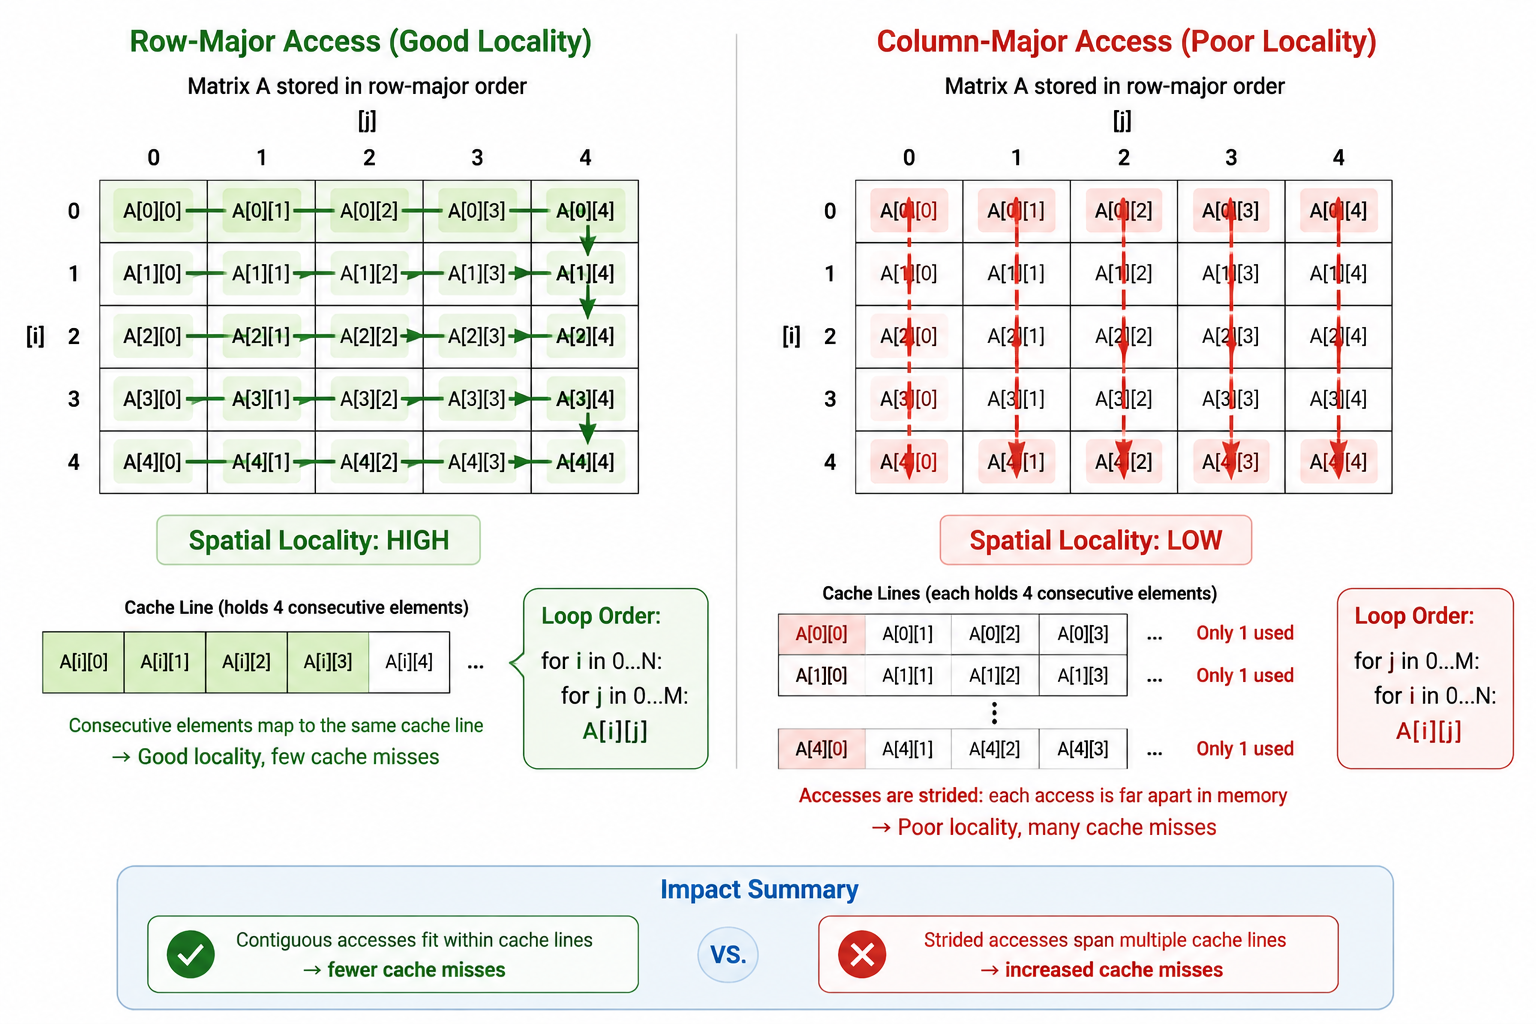
\includegraphics[width=1.0\textwidth]{ressources/chapter1/memory_access_patterns.png}    
    \caption{Effect of loop interchange on memory access patterns.}
    \label{fig:loop-interchange}
\end{figure}

\newpage
\subsection{Tiling}

Tiling partitions a large, multi-dimensional iteration space into smaller, localized blocks or sub-matrices called tiles. This structural change converts a deep loop nest of depth $D$ into a $2D$ structure composed of outer tile-traversal loops and inner point-execution loops.

In \gls{mlir}-\gls{rl}, this optimization is modeled as the \gls{t} action, where the framework identifies structural block dimensions, often chosen from a parameter space of powers of two. Figure~\ref{fig:loop-tiling} demonstrates how this geometric partitioning limits memory footprint size to dramatically optimize cache line retention.

\begin{itemize}
    \item \textbf{Mitigation of Capacity Misses:} Restricts the active computational working set to a compact footprint that fits entirely within high-speed cache tiers (L1/L2).
    \item \textbf{High-Bandwidth Data Reuse:} Drastically minimizes high-latency main memory traffic by keeping heavily accessed data elements close to the execution engine.
\end{itemize}

\begin{figure}[H]
    \centering
    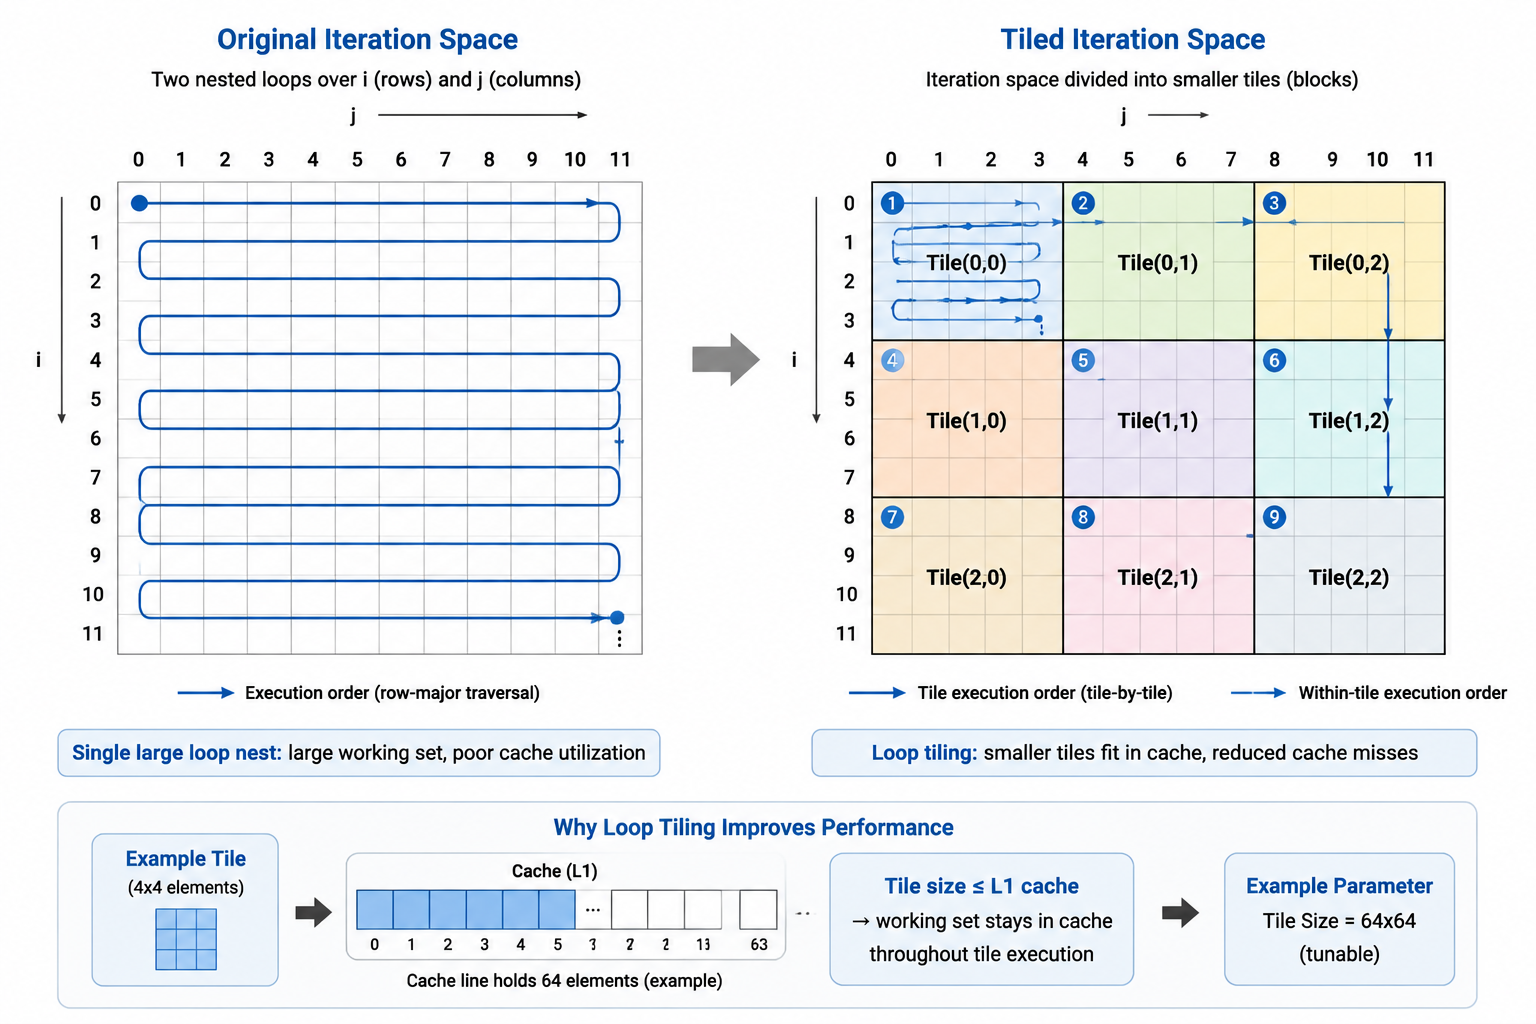
\includegraphics[width=1.0\textwidth]{ressources/chapter1/loop_tiling.png}
    \caption{Loop tiling and cache performance optimization.}
    \label{fig:loop-tiling}
\end{figure}

\subsection{Fusion}

Loop fusion merges two or more separate loops that share identical iteration bounds into a single, unified loop nest containing the bodies of all source loops. The transformation is legally valid only when there are no backward data dependencies between the distinct loops, ensuring the consumer loop does not require values computed by the producer in a future iteration.

In \gls{mlir}-\gls{rl}, this multi-operation optimization is mapped directly to the fusion action or combined into the multi-tier \gls{tf} action. The structural contraction of separate loop bodies into a localized execution pipeline is presented in Figure~\ref{fig:fusion-before}.

\begin{itemize}
    \item \textbf{Elimination of Intermediate Storage Overhead:} Replaces massive global memory buffers with temporary registers or L1 lines for direct producer-to-consumer data transfers.
    \item \textbf{Reduced Control Flow Overhead:} Compresses loop index tracking, branch instructions, and synchronization barriers across sequential computation blocks.
\end{itemize}

\begin{figure}[H]
    \centering
    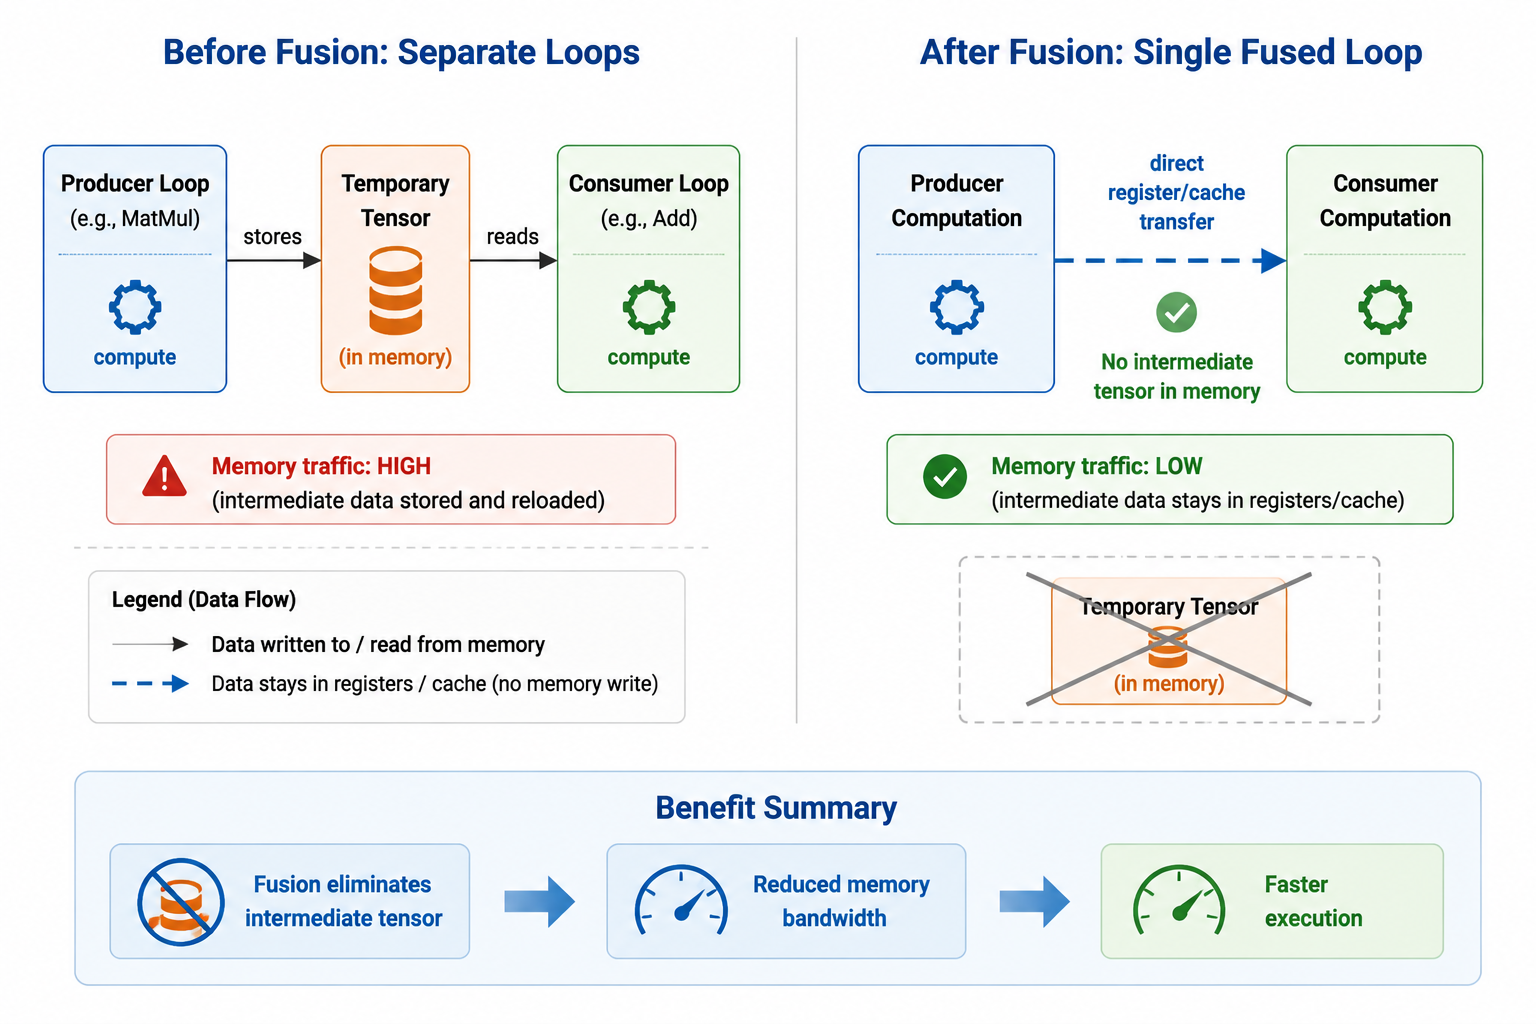
\includegraphics[width=0.9\textwidth]{ressources/chapter1/loop_fusion_comparison.png}
    \caption[Loop fusion]{Loop fusion: eliminating intermediate storage by merging producer and consumer loops.}
    \label{fig:fusion-before}
\end{figure}

\subsection{Vectorization}

Vectorization converts a standard scalar loop that processes one data element per iteration into a parallelized loop that executes operations on multiple uniform data elements simultaneously. This transformation relies on specialized execution units and wide microarchitectural hardware registers to process multiple values concurrently in a single clock cycle.

In \gls{mlir}-\gls{rl}, this is defined as the \gls{v} action, which frequently serves as a terminal action indicating that the schedule for a given operation is complete. Figure~\ref{fig:vectorization} directly contrasts this multi-element hardware processing paradigm with traditional sequential scalar execution lanes.

\begin{itemize}
    \item \textbf{Exploitation of Data-Level Parallelism:} Leverages low-level \gls{simd} instruction sets (e.g., AVX2, AVX-512) to significantly accelerate raw hardware compute throughput.
    \item \textbf{Compressed Instruction Count:} Minimizes the total volume of instructions fetched and decoded by the processor, reducing loop control branch overhead.
\end{itemize}

\begin{figure}[H]
    \centering
    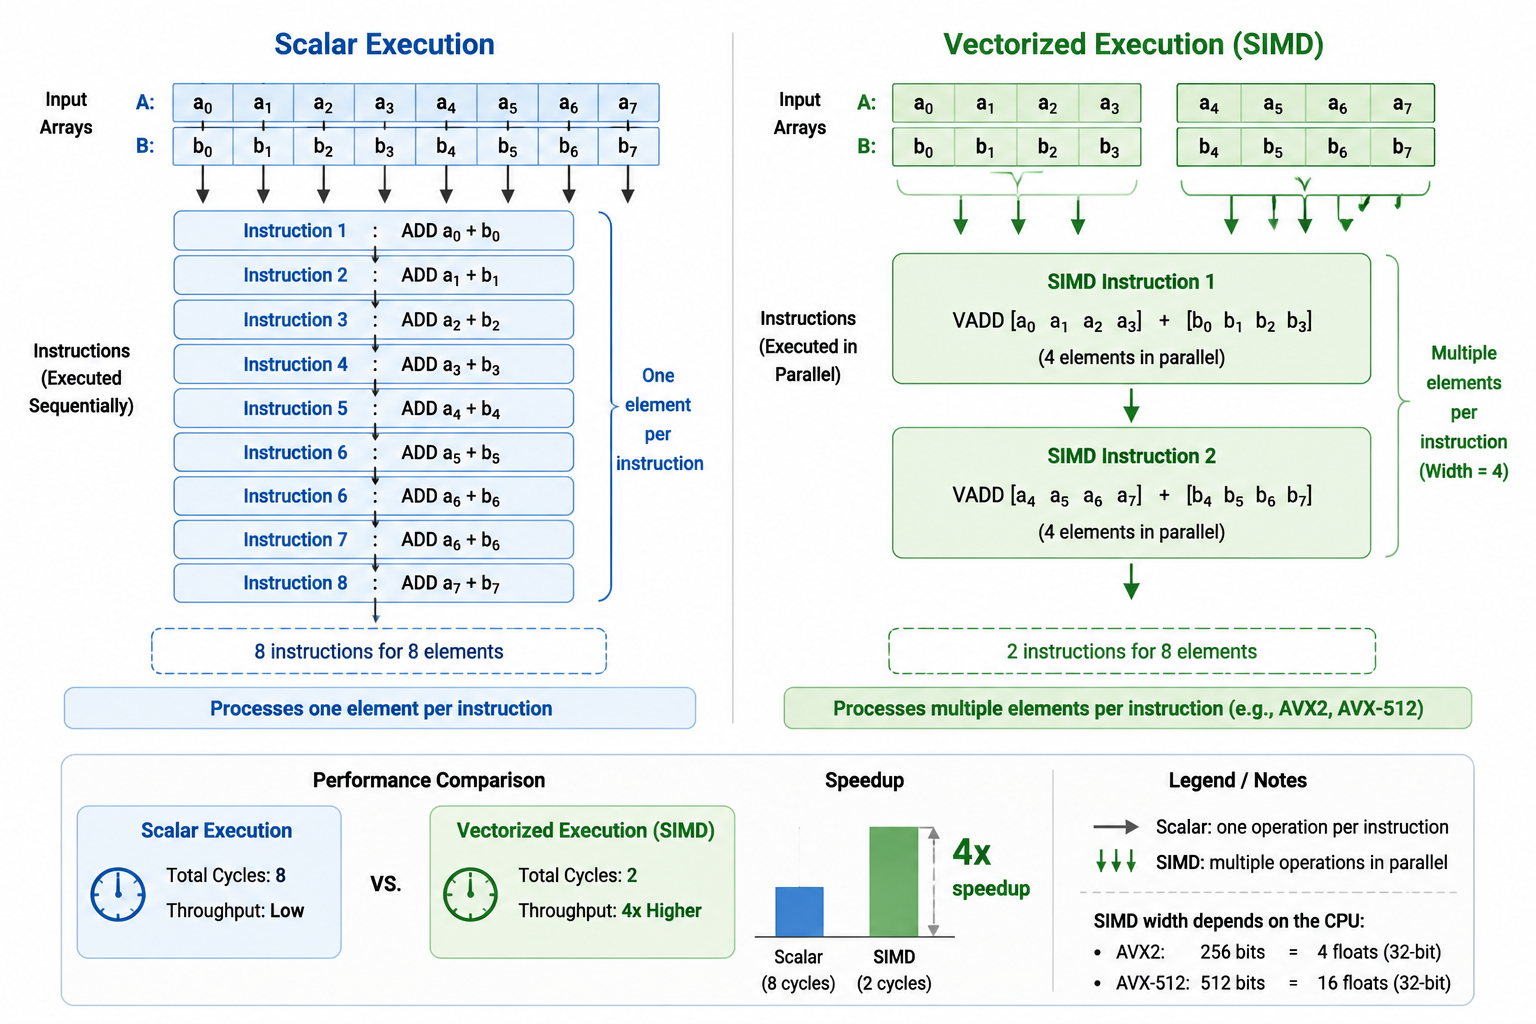
\includegraphics[width=1.0\textwidth]{ressources/chapter1/scalar_vs_SIMD_execution_comparison.png}
    \caption{Scalar vs SIMD execution comparison.}
    \label{fig:vectorization}
\end{figure}

To provide a comprehensive overview of the transformations discussed across this chapter, Table~\ref{tab:loop-transformations} synthesizes the core drivers, microarchitectural impacts, and legality criteria required for each distinct optimization strategy.

\begin{table}[H]
    \centering
    \caption{Summary of loop nest transformations covered in this chapter.}
    \label{tab:loop-transformations}
    \vspace{0.2cm}
    \begin{tabularx}{\textwidth}{l >{\raggedright\arraybackslash}p{3.5cm} >{\raggedright\arraybackslash}p{4cm} >{\raggedright\arraybackslash}p{4cm}}
        \toprule
        \textbf{Transformation} & \textbf{Mechanism} & \textbf{Primary Benefit} & \textbf{Legality Condition} \\
        \midrule
        Parallelization & Execute iterations concurrently & Reduced wall-clock time & No loop-carried dependencies \\
        \addlinespace
        Interchange & Swap loop nesting order & Improved memory locality & Dependence vectors remain valid \\
        \addlinespace
        Tiling & Partition iteration space into blocks & Cache utilization & No loop-carried dependencies \\
        \addlinespace
        Fusion & Merge producer-consumer loops & Eliminate intermediate storage & No backward dependencies \\
        \addlinespace
        Vectorization & Replace scalar ops with \gls{simd} & Instruction-level parallelism & Contiguous access, no dependencies \\
        \bottomrule
    \end{tabularx}
\end{table}

\section{Challenges in Modern Compiler Optimization}

Despite decades of research and engineering, several fundamental challenges make compiler optimization a difficult, open-ended problem.

\subsection{The Phase Ordering Problem}

The phase ordering problem is the challenge of determining the optimal sequence in which to apply compiler transformations~\cite{touati2014phase}. Transformations are not commutative: applying transformation $A$ before transformation $B$ can produce a different outcome than applying $B$ before $A$, because each transformation modifies the program in ways that affect the applicability and benefit of subsequent transformations.

For a concrete example, consider loop fusion and parallelization applied to a sequence of operations. If fusion is applied first, the two operations are merged, and the resulting combined loop can be parallelized. If parallelization is applied first, each operation is parallelized independently, and fusion may no longer be possible because the parallel loop structure differs. The choice between these two orders depends on the specific operation sizes, the cache hierarchy, and the available parallelism; there is no universally optimal order.

The search space of possible transformation sequences is combinatorial in the number of transformations and their parameters. For a loop nest with $D$ loops, there are $D!$ possible interchange permutations, $\mathcal{O}(T^D)$ possible tiling configurations (where $T$ is the number of tile size options), and an exponential number of interleavings between different transformation types. Exhaustive search is infeasible, and heuristics often fail to capture the interaction effects between transformations.

This combinatorial complexity directly motivates learning-based compilation frameworks like \gls{mlir}-\gls{rl}, where an optimization policy learns through experience and exploration which sequences of transformations are likely to be effective for a given program structure, bypassing the constraints of rigid heuristics. This structurally path-dependent discrepancy in downstream optimization outcomes is diagrammed explicitly in Figure~\ref{fig:phase-ordering}.

\begin{figure}[H]
    \centering
    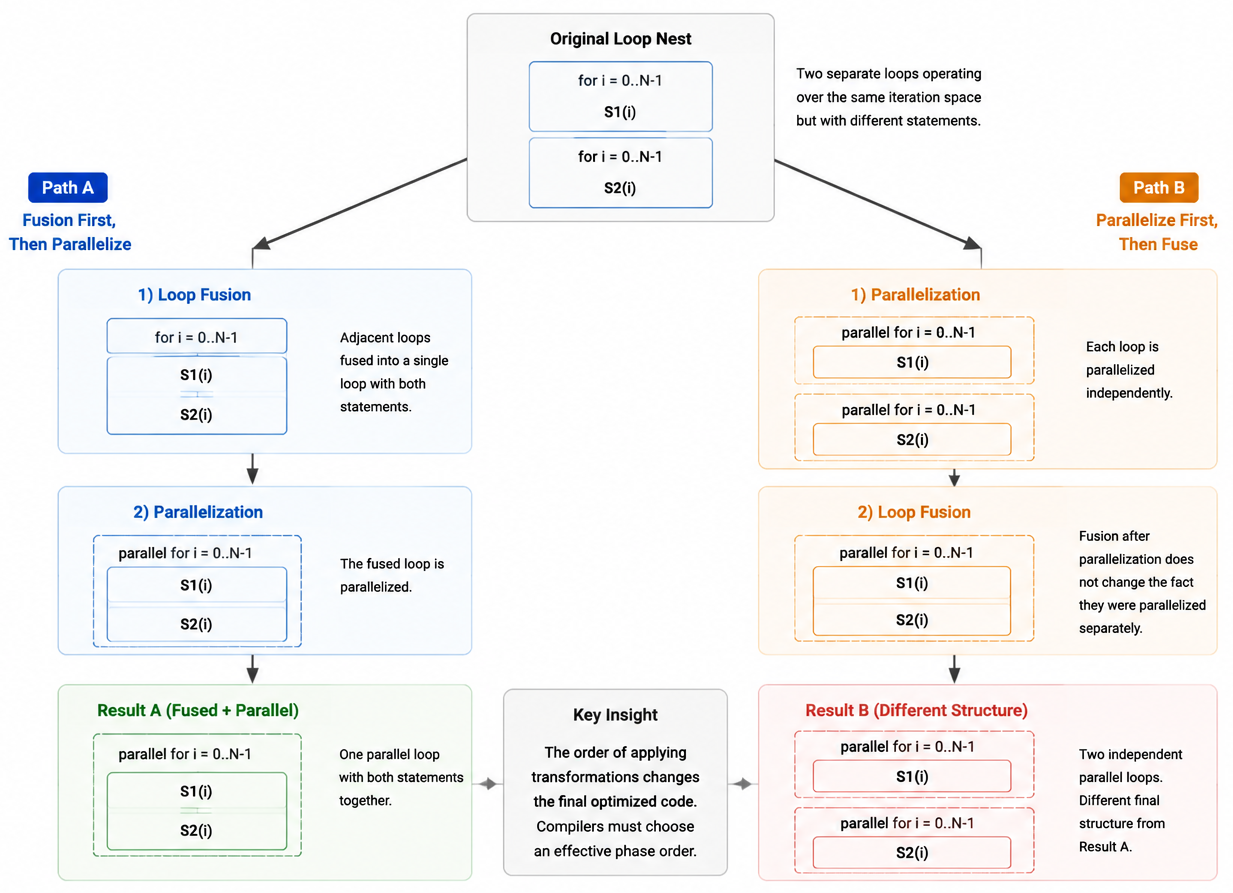
\includegraphics[width=1.0\textwidth]{ressources/chapter1/phase_ordering_problem.png}
    \caption{Phase ordering problem example.}
    \label{fig:phase-ordering}
\end{figure}

\subsection{Trade-offs}

Compiler optimization involves fundamental trade-offs between competing objectives:

\begin{itemize}
    \item \textbf{Performance vs.\ code size}: Optimizations such as loop unrolling and function inlining improve execution speed but increase the size of the generated code. On embedded systems with limited memory, code size may be the primary constraint.
    \item \textbf{Performance vs.\ compilation time}: More aggressive optimization analyses and search procedures take longer. For interactive development, fast compilation is preferred; for production deployment, longer optimization passes are acceptable.
    \item \textbf{Generality vs.\ specialization}: Optimizations tailored to specific program patterns (e.g., matrix multiplication of particular sizes) can achieve higher performance but do not transfer to new patterns. General-purpose optimizations apply broadly but leave performance on the table.
\end{itemize}

While performance optimization remains the primary objective of high-performance auto-scheduling systems, modern automated compilation pipelines frequently mitigate compilation time overheads through targeted strategies like evaluation caching, which records transformation outcomes to prevent redundant evaluations during exploration loops.

\subsection{Modern Hardware Integration}

The diversity and rapid evolution of hardware platforms add another dimension of complexity to compiler optimization. Modern computing environments include heterogeneous systems with \gls{cpu}, \gls{gpu}, \gls{npu}, and specialized accelerators, each with distinct memory hierarchies, instruction sets, and parallelism models. A transformation sequence that is optimal for one server architecture may be completely suboptimal for a different embedded or vector processor, even when compiling identical source routines. Some Hardware-aware solutions address this challenge by providing structural architectural specifications directly to the underlying decision model, allowing optimization pipelines to adapt flexibly across distinct deployment targets.

\section{MLIR Compiler Infrastructure}

The Multi-Level Intermediate Representation is a compiler infrastructure project within the \gls{llvm} compiler ecosystem, introduced by Lattner et al.~\cite{lattner2021mlir}. \gls{mlir} addresses a key limitation of traditional compiler \gls{ir}s: the assumption of a single, fixed level of abstraction. Traditional \gls{ir}s operate at one level (e.g., \gls{llvm} \gls{ir} operates close to machine code, while abstract syntax trees operate close to source code), making it difficult to express transformations that span multiple levels. \gls{mlir} instead supports a \textit{multi-level} \gls{ir}, where different \textit{dialects} define operations, types, and attributes at different levels of abstraction, all coexisting within the same representation.

\subsection{Dialects and Core Concepts}

A dialect in \gls{mlir} is a self-contained namespace of operations, types, and attributes that model a specific domain or abstraction level. \gls{mlir} ships with a set of core dialects that cover common compiler tasks. Table~\ref{tab:mlir-dialects} summarizes the primary dialects utilized throughout automated schedule generation pipelines.

\begin{table}[H]
    \centering
    \caption{Summary of core MLIR dialects used in this optimization domain.}
    \label{tab:mlir-dialects}
    \vspace{0.2cm}
    \begin{tabularx}{\textwidth}{l >{\raggedright\arraybackslash}p{5cm} >{\raggedright\arraybackslash}p{10cm}}
    
        \toprule
        \textbf{Dialect} & \textbf{Purpose} & \textbf{Optimization Context} \\
        \midrule
        Linalg & Structured linear algebra operations & Source representation of target benchmarks \\
        \addlinespace
        Affine & Polyhedral loops with affine constraints & Intermediate lowering; dependence analysis \\
        \addlinespace
        \gls{scf} & Structured control flow (for, if, forall) & Loop representation after lowering \\
        \addlinespace
        \gls{llvm} & Direct mapping of \gls{llvm} \gls{ir} in \gls{mlir} & Final stage before \gls{jit} compilation \\
        \addlinespace
        Transform & Transformation schedule encoding & Mechanism for applying structured actions \\
        \bottomrule
    \end{tabularx}
\end{table}

An \gls{mlir} module is a container for operations, which may themselves contain regions of nested operations. This hierarchical structure, combined with the dialect system, allows the same module to contain Linalg operations describing a neural network layer, vector operations representing the \gls{simd} instructions generated for that layer, and \gls{llvm} operations ready for code generation, all within a single, coherent representation. This multi-tier lowering sequence across distinct dialect abstraction thresholds is systematically traced in the flowchart mapping shown in Figure~\ref{fig:mlir-dialect-stack}.

\begin{figure}[H]
    \centering
    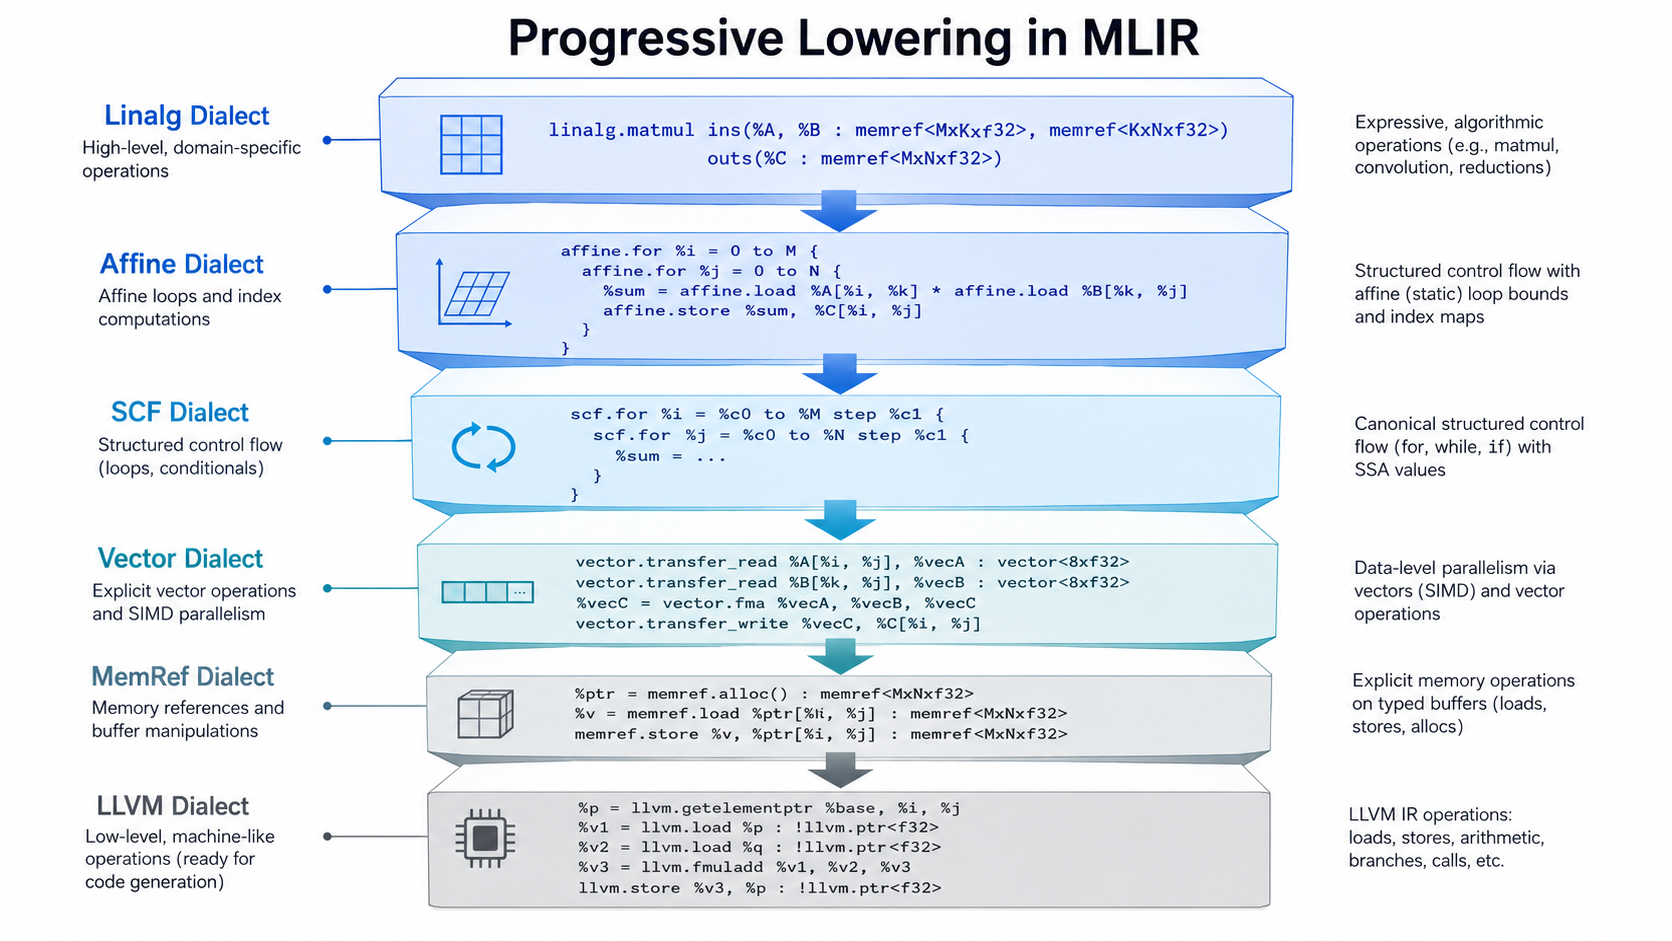
\includegraphics[width=1.0\textwidth]{ressources/chapter1/progressive_lowering_MLIR.png}
    \caption{Progressive lowering in MLIR flowchart.}
    \label{fig:mlir-dialect-stack}
\end{figure}

\subsection{MLIR Pipeline for Automated Optimization and Evaluation}

Several properties of \gls{mlir} make it uniquely well-suited for integration into automated optimization workflows, particularly those utilizing reinforcement learning or heuristic engines:

\begin{enumerate}
    \item \textbf{Explicit loop structure}: Linalg operations explicitly encode structural loops, memory access patterns, and mathematical calculations, providing an informative representation of the optimization target.
    \item \textbf{Progressive lowering}: \gls{mlir} supports the gradual lowering of operations through the dialect stack, moving cleanly from high-level mathematical descriptions down to target-specific assembly abstractions.
    \item \textbf{Python bindings}: Comprehensive Python bindings allow compilation frameworks to query, manipulate, and execute \gls{mlir} modules programmatically. This integrates seamlessly with modern learning libraries. The bindings also expose the transform dialect interpreter, which handles precise code schedules systematically.
    \item \textbf{Extensibility}: New dialects and transformations can be added to \gls{mlir} without modifying the core infrastructure.
\end{enumerate}

These architectural advantages directly enable the practical execution pipeline required to evaluate compiler transformation sequences. To measure performance impact dynamically, the target \gls{mlir} module is processed through lowering passes to the \gls{llvm} dialect, translated to standard \gls{llvm} \gls{ir}, and \gls{jit}-compiled using \gls{mlir}'s ExecutionEngine. Finally, the compiled function is invoked through a timed wrapper to gather exact hardware execution cycles or runtime speedups. This closed-loop process serves as the underlying evaluation and feedback mechanism for calculating reward signals and fitness functions within learning loops.
\section{Conclusion}

This chapter established the foundational compiler concepts of this thesis, surveying the traditional three-phase compilation pipeline, hardware-dependent and independent optimization paradigms, and safety-guaranteeing control-flow and data-flow analyses.

It detailed key loop nest transformations mapping their underlying mechanics to localized \gls{mlir}-\gls{rl} actions. These techniques directly target the structural and memory-bound bottlenecks characteristic of compute-intensive workloads.

The discussion then examined the primary limitations of hand-crafted compilation heuristics: the combinatorial complexity of the phase ordering problem, conflicting microarchitectural design trade-offs, and accelerating hardware heterogeneity. These challenges underscore the necessity for automated alternatives.

Finally, the \gls{mlir} framework was introduced as an ideal ecosystem for learning-based optimization, leveraging its multi-level dialect stack (notably Linalg and Transform), explicit loop semantics, and Python bindings. The vast, non-commutative search spaces identified here directly motivate the reinforcement learning approach detailed in the next chapter.
